\documentclass{exos}
\usepackage{main}

\title{Activite : Croissance exponentielle}
\author{Première Spécialité Mathématique}
\date{Chapitre 7 Partie 3}

\begin{document}
\maketitle

Dans un parc naturel, le nombre de loutres recensé augmente chaque année de \num{1.6}\%. En 2020, le nombres d'individu est de \num{1864}.

On modélise par une suite $(u_n)$ le nombre de loutres lors de l'année $2020 + n$.

\begin{alphaquestions}
\item Donner $u_0$; $u_1$ et $u_2$.
\item Justifier que la suite $(u_n)$ est géométrique, en précisant sa raison.
\item En déduire que l'expression du terme $u_n$ en fonction de $n$ est donné par
\begin{equation*}
u_n = 1864 \times 1,016^n
\end{equation*}
\item On donne la courbe de la fonction exponentielle $x \mapsto e^x$.
\begin{center}
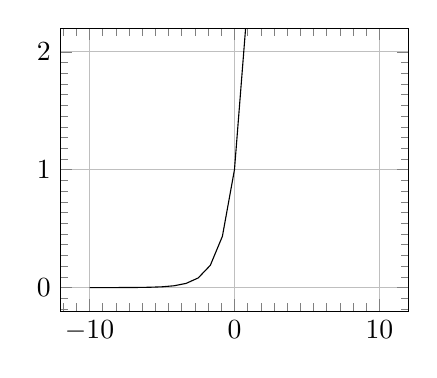
\begin{tikzpicture}
\begin{axis}[xmin=-10,xmax=10,ymin=0,ymax=2,restrict y to domain=-1:3,enlargelimits,width=6cm,grid=major,minor tick num=10]
\addplot[domain=-10:10] {e^x};
\end{axis}
\end{tikzpicture}
\end{center}
Conjecturer le nombre de solutions à l'équation $e^x = 1,016$.
\item On note $a$ une telle solution (donc $e^a = 1,016$). En déduire qu'une expression de $u_n$ en fonction de $n$ est donnée par
\begin{equation*}
u_n = 1864 \times e^{an}
\end{equation*}
\item On souhaite étudier l'évolution de cette population de loutre à chaque instant (et pas seulement chaque année). Pour cela, on pose la fonction
\begin{equation*}
\function{f}{\R}{\R}{x}{1864 \times exp(ax)}
\end{equation*}
Pour quelle valeur de $x$ la fonction $f(x)$ prend la valeur $u_0$ ? Et $u_1$ ?
\item Quelle valeur de $x$ choisir pour que $f(x)$ corresponde à la population de l'autre au bout de \num{6} mois (une demi-année).
\item Même question pour \num{3} mois ?
\end{alphaquestions}
\end{document}